In this section we present our data on the expected number of ballots drawn as the number of rounds increases, and on the fraction of audits that stop (an estimate of cumulative stopping probability, $C_j$) for the states of Texas, Missouri and Massachusetts, with margins of $0.057$, $0.157$ and $0.342$ respectively. Interestingly, we observe that the advantage $\Minerva$ has for a first round size with stopping probability $S_1=0.9$ is retained for $S_1=0.25$. 

\begin{figure}
\begin{centering}
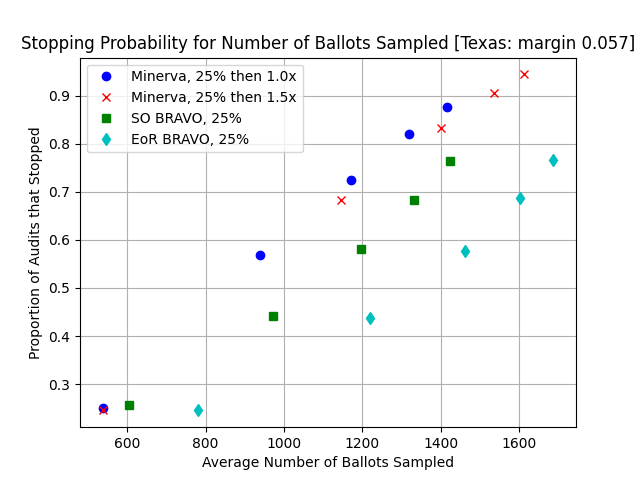
\includegraphics[width=0.75\textwidth]{texas2.png}
\caption{This plot shows the cumulative fraction of audits that stopped as a function of average number of sampled ballots for all four audits we studied, for the state of Texas, margin $0.057$, and first round stopping probability $S_1=0.25$.}
\label{fig:texas_25}
\end{centering}
\end{figure}

We observe that the behavior of both \Minerva audits is similar, and that the plot for SO \BRAVO is to the right (more ballots) and below (lower probability of stopping) those for \Minerva, even for a stopping probability as low as $0.25$. We observe that the plot for EoR \BRAVO shows the worst performance, which is not surprising. We observe similar behavior across margins (see Figures \ref{fig:missouri_25} and \ref{fig:mass_25}), though the improvement due to \Minerva reduces margins get larger. We see also that the behavior is similar to that seen for $S_1=0.9$ (see Figure \ref{fig:texas_90}). 

\begin{figure}
\begin{centering}
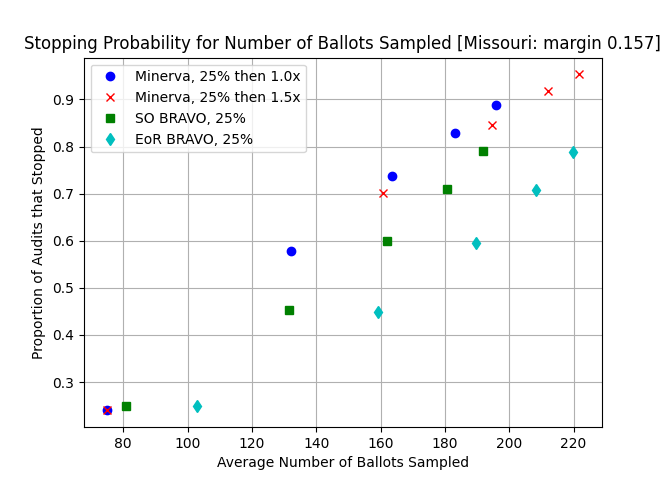
\includegraphics[width=0.75\textwidth]{missouri2.png}
\caption{This plot shows the cumulative fraction of audits that stopped as a function of average number of sampled ballots for all four audits we studied, for the state of Missouri, margin $0.157$, and first round stopping probability $S_1=0.25$.}
\label{fig:missouri_25}
\end{centering}
\end{figure}

\begin{figure}
\begin{centering}
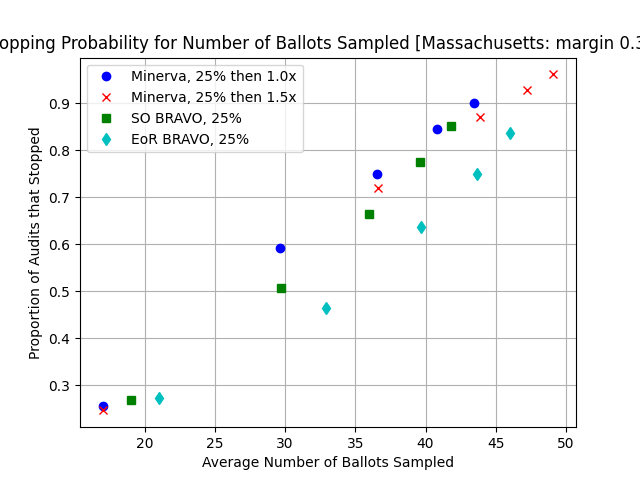
\includegraphics[width=0.75\textwidth]{massachusetts2.png}
\caption{This plot shows the cumulative fraction of audits that stopped as a function of average number of sampled ballots for all four audits we studied, for the state of Massachusetts, margin $0.342$, and first round stopping probability $S_1=0.25$.}
\label{fig:mass_25}
\end{centering}
\end{figure}

\begin{figure}
\begin{centering}
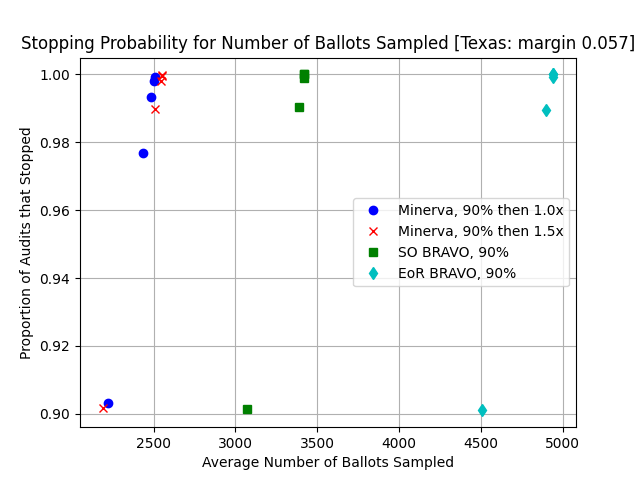
\includegraphics[width=0.75\textwidth]{texas1.png}
\caption{This plot shows the cumulative fraction of audits that stopped as a function of average number of sampled ballots for all four audits we studied, for the state of Texas, margin $0.057$, and first round stopping probability $S_1=0.9$.}
\label{fig:texas_90}
\end{centering}
\end{figure}

